\section{Experiment 1: Quadratic Voting, Likert scale surveys, and Donation}
\subsection{Methodology} \label{method-1}
% Experiment overview
We designed the first experiment 
consisting of Likert survey, QV, and a donation task,
to answer research questions one and three. 
Participants were recruited from Amazon Mechanical Turk (MTurk)
with 213 valid submissions. %screens 3.4K 
They received \$0.75 and \$1.75 according to the groups they are assigned to.
In this section, 
we detailed our experiment design.

%The donation task. Why?
In order to figure out 
how QV and Likert surveys 
represent an individual's true preferences,
we ask participants to complete a survey
and donate to a charity.
Our goal is to see 
whether a participant's donation behavior is similar to 
the attitudes they stated in the survey.
There are multiple reasons
why we designed a donation task.
First, donation tasks are easily relatable
given that they occur in real life and
and monetary behaviors are direct and imaginable.
Second, donations are simple to conduct,
even on a large scale.
Third, donation tasks appeared in many experiments 
\cite{Xiao2019, benz2008people, gendall2010effect} 
as an effective indicator of participants' behavior.
Fourth, donating is a behavior containing
complimentary and homogenous choices and
where each of the options is independent.
It is a clear example of choosing one out of $K$ in real life.

\begin{figure}[htpb]
    \centering
    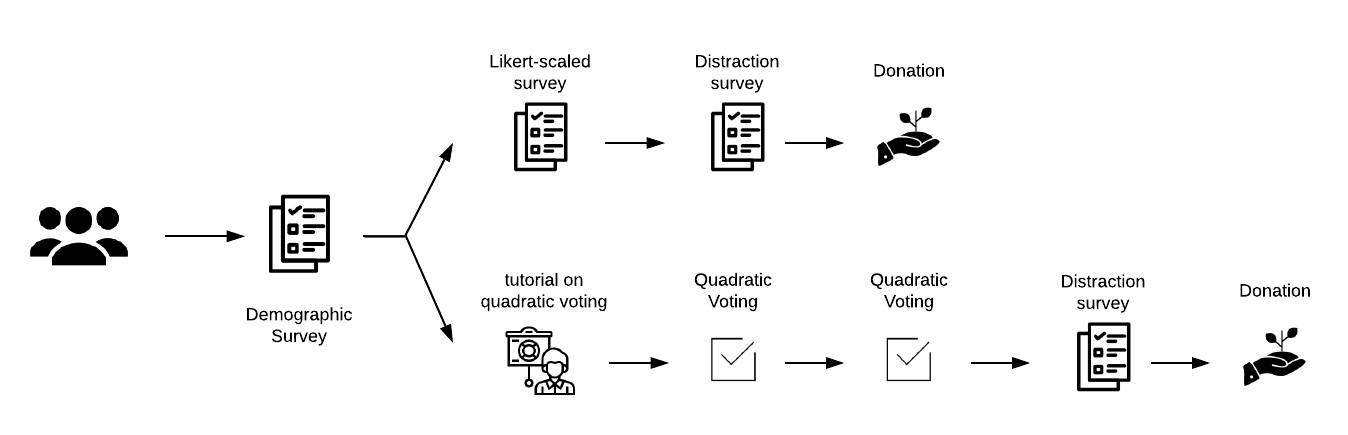
\includegraphics[width=\textwidth, keepaspectratio=true]{content/image/exp1_flow.png}
    \caption{
        Experiment one conducted between subjects. Participants were divieded into two groups. Participants that took the upper path is the Likert Group and the alternative is the QV group.
    }
    \Description[Image describing the flow for experiment 1]{Image describing the flow for experiment 1}
    \label{fig:exp1_image_flow}
\end{figure}

At a high level, 
we summarize the experiment flow 
in Graph \ref{fig:exp1_image_flow}.
The experiment consisted of four steps:
To begin the experiment, 
participants filled out the demographic survey.
Based on the demographics,
participants completed one form of opinion collection,
highlighted as the yellow box
in Graph \ref{fig:exp1_image_flow}.
After that, 
participants filled out another survey,
the distraction survey,
to divert their attention before they complete the final task.
The final task asked participants to donate.
Now we explain each section in detail.

Before starting the experiment,
participants were told that 
this study aims to understand their opinions 
toward social causes and will be asked to complete a donation task.
During the demographic survey, 
we collected the participant's gender, ethnicity, age range, household income level, 
education level, and current occupation.
Based on the age and education level,
we divided participants into seven groups
and made sure each group contained the same distribution
as the US 2019 census.
These seven groups can be further categorized as
the Likert Group (Group 1) and the QV Group (Group 2 to 7).
The Likert Group, shown as the upper path in the shaded area of Graph \ref{fig:exp1_image_flow}, 
revealed their opinion using a Likert scale survey.
The QV Group, shown as the lower path in the shaded area of Graph \ref{fig:exp1_image_flow}, 
revealed their opinions by completing two QVs, each with different numbers of voice credit.
We divided the QV Group into six subgroups
to answer research question three, 
which is whether the number of voice credits impacts the outcome.
These two voice credits that participants experience 
are drawn from three possible values: $N \times O$, $N^1.5 \times O$, $N^2 \times O$, 
where $N$ is the number of options in the survey, 
and $O$ is the number of levels, 
excluding neutral on the Likert scale survey. %not sure if this is clear
In our case, with nine options ($N=9$) and
used a five-point Likert scale survey ($O=4$), 
the three values would be $36$, $108$, and $324$.
With these three possible values, 
we choose two for each of the six subgroups.

In the Likert group, 
the survey looks identical to a typical five-point Likert scaled survey.
We assume participants have prior knowledge in Likert surveys.
Participants were presented with the nine societal causes, 
and were asked the importance each of these causes: 
With options ranging from ``Very important'' to ``Very Unimportant.''

In the QV group, 
participants were asked to watch 
a prerecorded tutorial video of QV's concept 
and how to operate the QV interface.
Participants are granted unlimited time 
to interact with a demo QV interface. 
This process is demonstrated as 
``tutorial on quadratic voting'' 
in Graph \ref{fig:exp1_image_flow}.
To ensure that participants paid attention to the video and understood QV, 
they were asked to answer at least three of the five multiple-choice questions 
correctly to continue with the survey.
Once participants passed the quiz, 
participants will be given voice credits of either 36, 108, or 324.
They will vote in QV using these voice credits 
with the nine options identical to those in the Likert Group.
Participants would repeat this action using a different set of voice credits.
These two QVs are shown as two QV icons in Graph \ref{fig:exp1_image_flow}.



After both groups of participants completed their surveys in the opinion collection stage, 
they finish a short answer question
that allowed them to express their thoughts 
related to another set of societal issues.
These societal issues are unrelated in the previous stage,
and are designed to distract participants.
We do not want participants to connect their survey responses
to interfere with their behaviors during the donation task.

Finally, 
we ask participants to perform a donation in the final stage.
This task presented nine organizations,
each referring to one of the nine societal causes
that we listed during the opinion collection phase.
Participants can donate up to 35 dollars 
to any of these organizations.
To ensure incentive compatibility, 
participants do not donate imaginatively.
Participants are aware that every one in 70 participants would win 35 US dollars.
Assuming winning the 35 US dollars, 
the participants were asked 
if they would want to donate some money 
to any of the nine charity groups.
Participants are also aware that 
they keep the remaining amount of undonated money 
if they win the lottery.
Further, participants are aware that 
the research team will match one dollar to each one dollar 
they donated to an organization.
This setup means the donation carried an underlying cost.

To minimize the difference across groups in the study, 
we use the same prompt across Likert scaled survey, QV, and the donation task.
We explicitly tell the participants that 
there are limited resources in the society, 
and people have different preferences 
in how resources should be allocated and ask the participants, 
``What societal issues need more support?''

To ensure that the nine societal causes 
covered a broad spectrum of categories.
We used the categorization of charity groups on Amazon Smile, 
a popular donation website that has accumulated over 100 million dollars of donations, 
as our topics of the societal causes.
The categories include (1) Pets and Animals, (2) Arts, Culture, Humanities, (3) Education, (4) Environment, 
(5) Health, (6) Human Services, (7) International, (8) Faith and Spiritual, and (9) Veteran. 
Within each of these categories, 
we select one charity organization from Amazon Smile 
as the representation of the subject matter used in the donation task.

\subsection{System Design}
We use Python Flask for the back-end, Angular for front-end, 
and MongoDB for database storage to construct the voting system. 
The experiment source code is publicly available \footnote{Not yet public}, 
and so is the QV interface as a stand-alone repository \footnote{https://github.com/hank0982/QV-app}.

\begin{figure}[htpb]
    \centering
    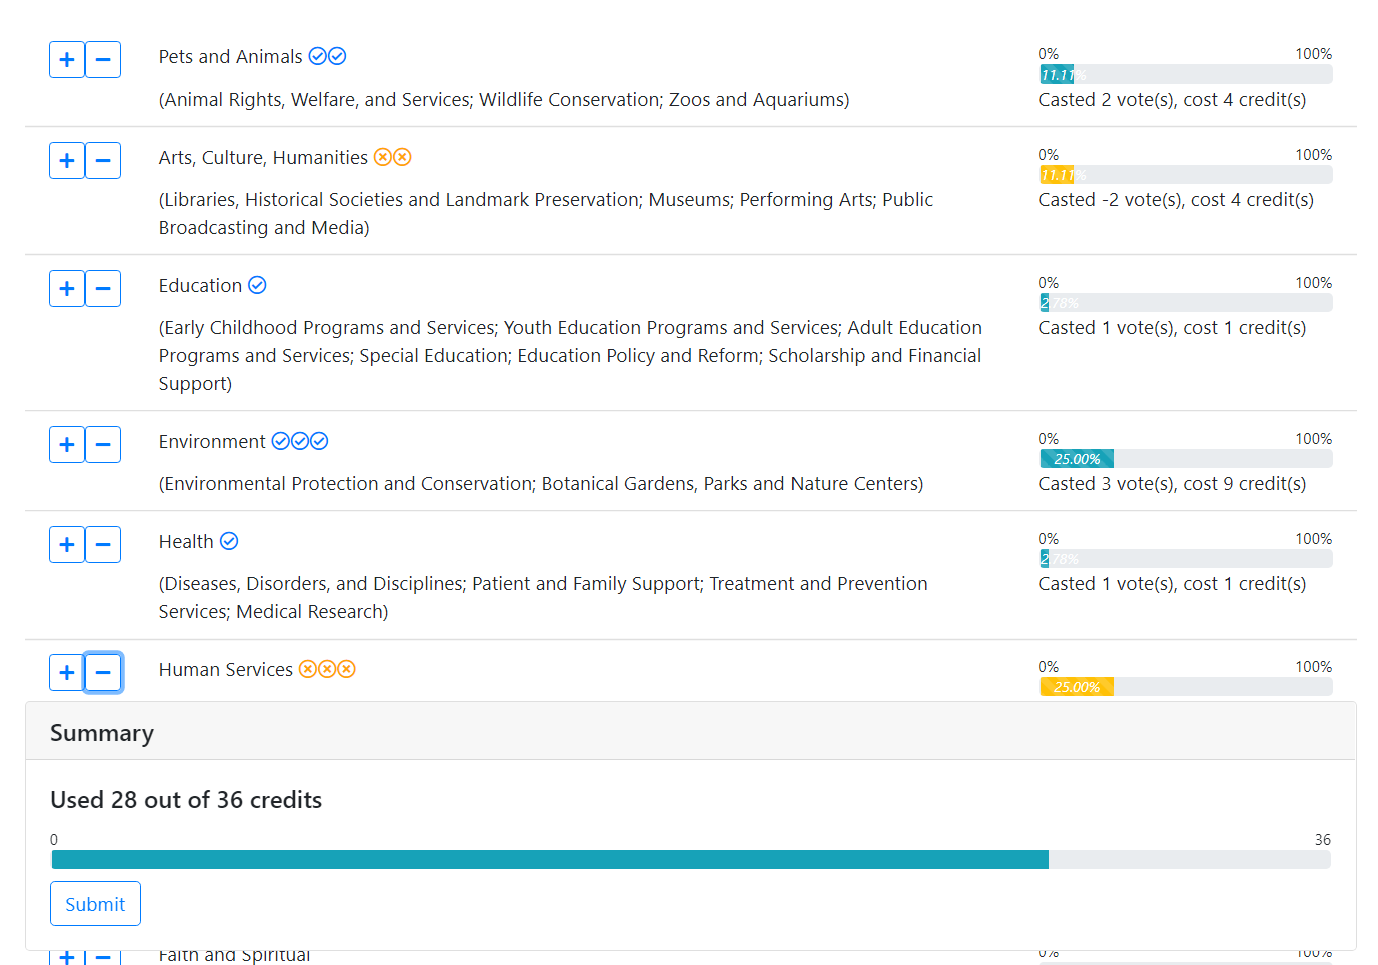
\includegraphics[width=0.7\textwidth, keepaspectratio=true]{content/image/qv-donation.png}
    \caption{
        The QV voting interface used across both experiments. 
        We omit the prompt in this figure.
        After mutiple iterations (details in the Appendeix), 
        the interface allows participants to vote, 
        with real time feedback of how the votes allocats. 
        The progress bar implementation 
        were inspired by knapsack voting interface by \textcite{goel2015knapsack}.
    }
    \label{fig:qv_donation}
\end{figure}

The QV interface, is shown in Figure \ref{fig:qv_donation}.
The body section is the voting panel
that contained all options to vote for.
To the left of each option, 
participants vote using the plus and minus buttons.
Buttons are disabled 
if the number of voice credits 
does not permit the next vote.
A bar on the right of the option 
shows the proportion of voice credits 
used to that option with text associated with the visual.
The different colors and the icons 
to the right of each option 
exhibits the number of for or against 
that currently devoted to an option.
The summary panel always 
floats at the bottom of the page 
to ensure visibility.
A progress bar shows the number of voice credits 
that the participants have and had not used.\par